\section{Results} \label{results}

In this section, we first discuss the performance of the trained \ac{RF} and \ac{KNN} classifiers on the testing data set $D_S$ and use the latter to calculate the Bayesian probabilities
$P_M(I|{\bf A})$. Then we evaluate $P_M(I|{\bf A})$ on two independent data sets. The first set includes a population of simulated \ac{CBC} events that were injected in the real-time
replay of \ac{O3} data and was used for the \ac{LVK} \ac{MDC}~\cite{Chaudhary:2023vec}. The second set contains the confident \ac{LVK} \ac{O3} detections that are reported in \ac{LVK}'s
\ac{GWTC3} catalog~\cite{LIGOScientific:2021djp}.

\subsection{Performance on the O2 Testing Set}

We assess the performance of the classifiers by measuring the \ac{TPR} and the \ac{FPR} of the events in $D_S$. We present our findings as \ac{ROC} curves that illustrate how the \ac{TPR}
varies for various score thresholds as a function of the \ac{FPR}.

\begin{figure*}%[h]
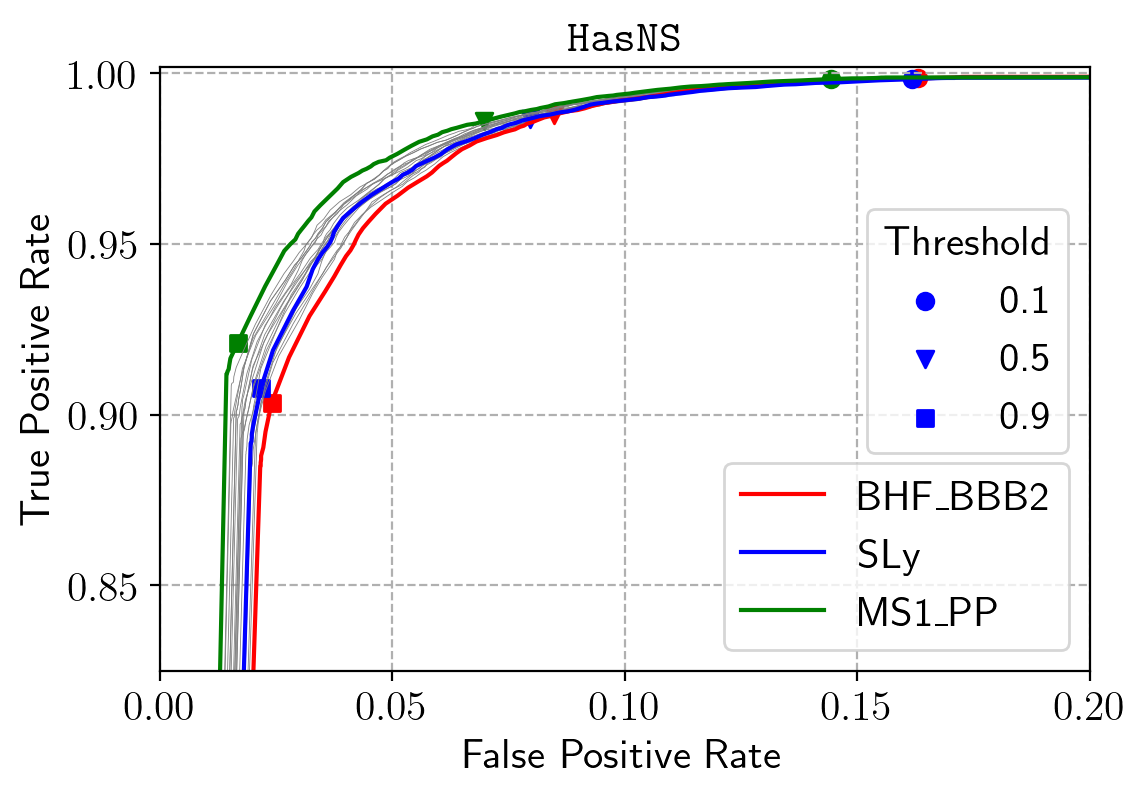
\includegraphics[width=0.47\linewidth]{roc_testing_KNN_NS}
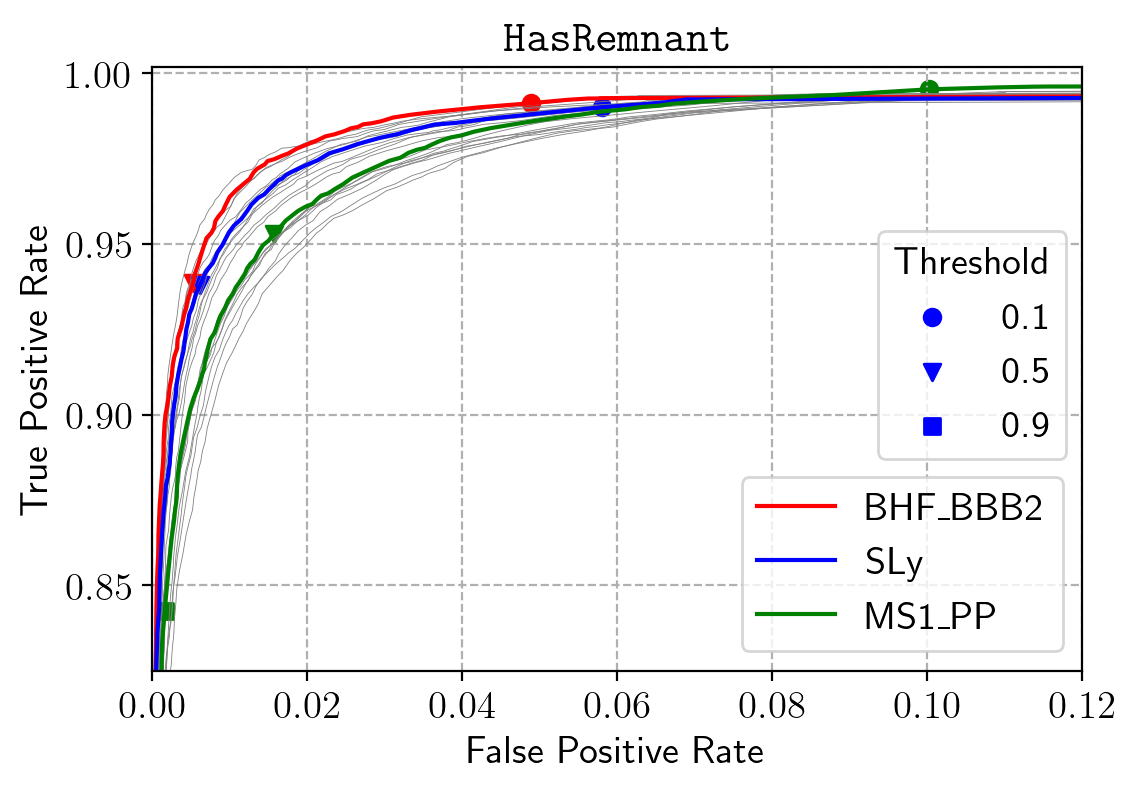
\includegraphics[width=0.45\linewidth]{roc_testing_KNN_REM}
\caption{\ac{ROC} curves obtained from the \ac{O2} testing data set $D_S$ for the \ac{KNN} classifier (left: \hasns, right: \hasrem). The curves for the 23 different \ac{EOS}s are displayed in
gray, with the curves for {\tt BHF\_BBB2}, {\tt MS1\_PP}, and {\tt SLy} highlighted in red, green, and blue, respectively. The circle, triangle, and square markers denote score thresholds of
$0.1$, $0.5$, and $0.9$, respectively.}
\label{fig:rocO2_KNN}
\end{figure*}

\begin{figure*}%[h]
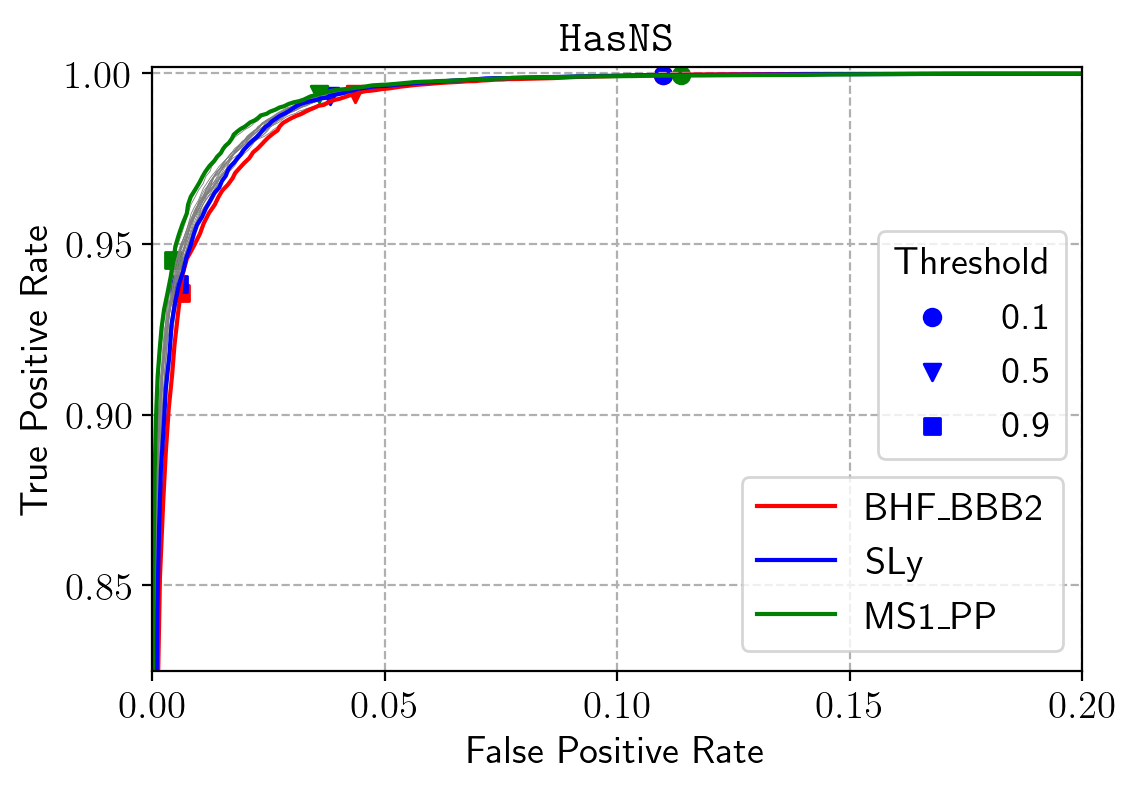
\includegraphics[width=0.47\linewidth]{roc_testing_RF_NS}
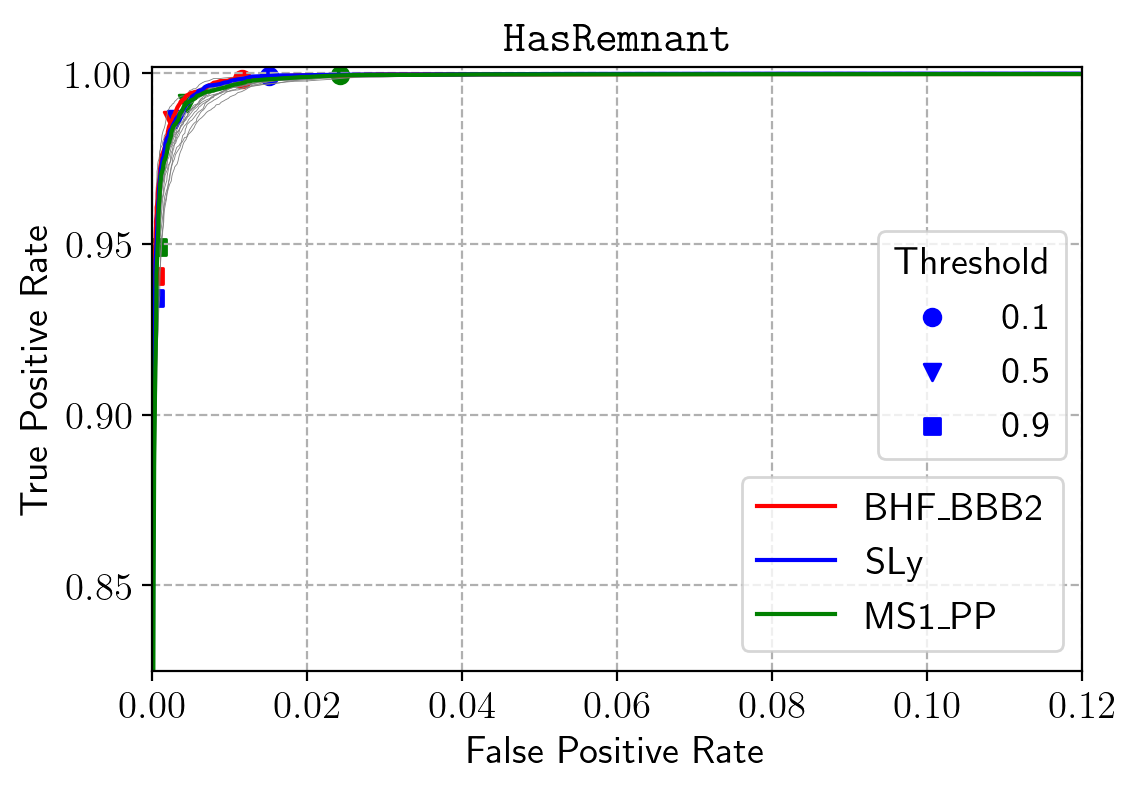
\includegraphics[width=0.45\linewidth]{roc_testing_RF_REM}
\caption{\ac{ROC} curves obtained from the \ac{O2} testing data set $D_S$ for the \ac{RF} classifier (left: \hasns, right: \hasrem). The curves for the 23 different \ac{EOS}s are displayed in
gray, with the curves for {\tt BHF\_BBB2}, {\tt MS1\_PP}, and {\tt SLy} highlighted in red, green, and blue, respectively. The circle, triangle, and square markers denote score thresholds of
$0.1$, $0.5$, and $0.9$, respectively.}
\label{fig:rocO2_RF}
\end{figure*}

The \hasns\ and \hasrem\ \ac{ROC} curves for the  \ac{KNN} algorithm are displayed in the left and right panels of Fig.~\ref{fig:rocO2_KNN}, respectively. Figure \ref{fig:rocO2_RF}
displays the analogous curves for the \ac{RF} classifier. The \ac{ROC} curves for the 23 \ac{EOS} are plotted in gray, with three of them highlighted in color: {\tt BHF\_BBB2}, the
\ac{EOS} with the lowest maximum mass for the NS; {\tt MS1\_PP}, the \ac{EOS} with the largest maximum mass for the \ac{NS}; and {\tt SLy}, which allows for a maximum mass of $2.05
M_\odot$ and is the standard \ac{EOS} used in \ac{LVK} low-latency investigations~\cite{Ghosh:2021eqv}. The markers denote different thresholds for the algorithm scores. 

The two classifiers perform consistently across all \ac{EOS}s. The \ac{TPR} for a score threshold of $0.5$ is around $0.99$ for both \hasns\ and \hasrem. A comparison of the \hasns\ and
\hasrem\ \ac{ROC} curves for each algorithm shows that the \ac{FPR} for \hasns\ is generally higher than the \ac{FPR} for \hasrem\ at a given threshold. Thus, the algorithms typically do
a better job in classifying \hasrem\ than \hasns. Separate comparisons of the \ac{KNN} and \ac{RF} \ac{ROC} curves for \hasns\ and \hasrem\ reveal that at a given threshold, \ac{RF}
produces slightly higher \ac{TPR} and lower \ac{FPR} than \ac{KNN}.

\subsection{Bayesian Probabilities for the O3 Sets}

After the algorithms have been trained and tested, we compute the Bayesian probabilities defined in Sec.~\ref{bayesian_probs} in terms of their outcomes. Equations~\eqref{bayes-hasns} and
\eqref{bayes-hasrem} must be assessed on a data set independent of the training data set, as stated in Sec.~\ref{bayesian_probs}. To do so, we employ $D_S$.

\begin{figure*}%[h]
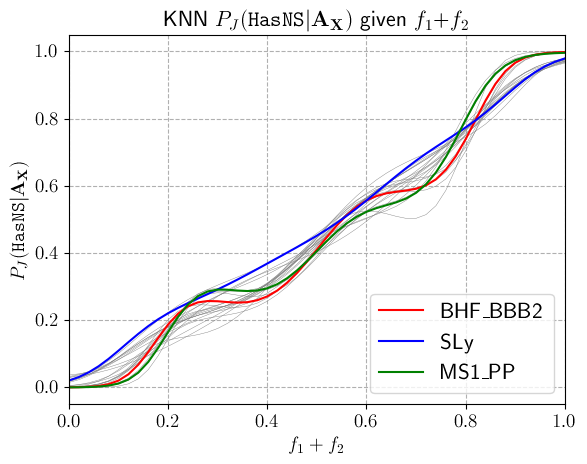
\includegraphics[width=0.45\linewidth]{KNN_3_eos_prob_plots_HasNS}
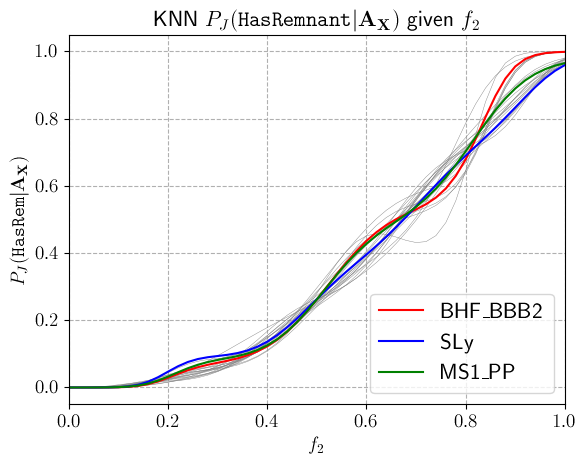
\includegraphics[width=0.45\linewidth]{KNN_3_eos_prob_plots_HasRem}
\caption{Left panel: \hasns\ Bayesian probability curves for the 23 \ac{EOS} as a function of the fraction of \ac{KNN} neighbors $f_1+f_2$. Right panel: \hasrem\ Bayesian probability curves as a function of the fraction of \ac{KNN} neighbors $f_2$. Curves for the {\tt BHF\_BBB2}, {\tt MS1\_PP}, and {\tt SLy} \ac{EOS}s are highlighted in red, green, and blue, respectively. The probabilities show an increasing trend as the fraction of neighbors increases. Non-monotonic fluctuations are due to the data set's finite size.}
\label{fig:bayesian_prob_fits_KNN}
\end{figure*}

\begin{figure*}%[h]
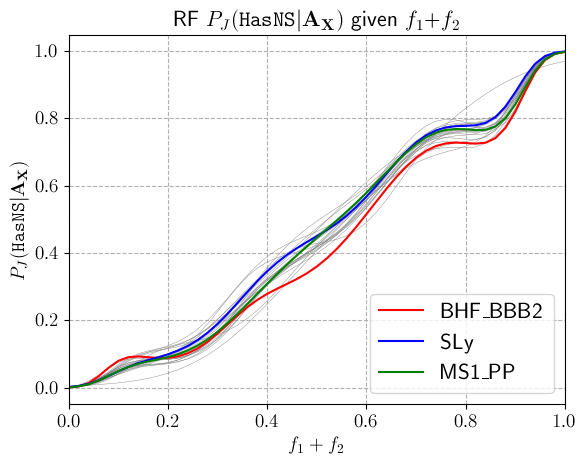
\includegraphics[width=0.45\linewidth]{RF_3_eos_prob_plots_HasNS}
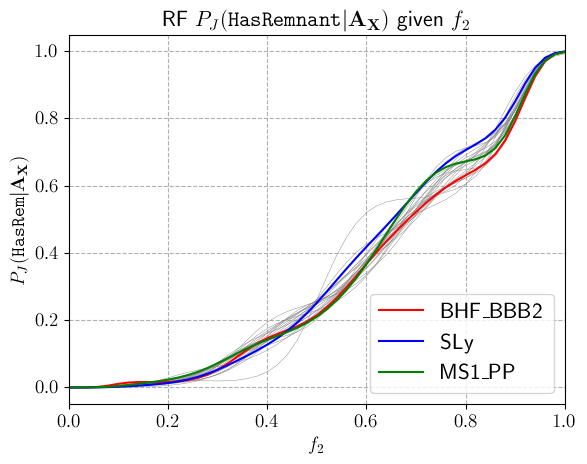
\includegraphics[width=0.45\linewidth]{RF_3_eos_prob_plots_HasRem}
\caption{Left panel: \hasns\ Bayesian probability curves for the 23 \ac{EOS} as a function of the fraction of \ac{RF} trees $f_1+f_2$. Right panel: \hasrem\ Bayesian probability curves for \hasrem\ as a function of the fraction of \ac{RF} Trees $f_2$. Curves for the {\tt BHF\_BBB2}, {\tt MS1\_PP}, and {\tt SLy} \ac{EOS}s are highlighted in red, green, and blue, respectively. The probabilities show an increasing trend as the fraction of trees increases.  Non-monotonic fluctuations are due to the data set's finite size.}
\label{fig:bayesian_prob_fits_RF}
\end{figure*}

The \ac{KNN} and \ac{RF} probability estimators are shown for each of the 23 \ac{EOS} in Figs.~\ref{fig:bayesian_prob_fits_KNN} and~\ref{fig:bayesian_prob_fits_RF}, respectively. As
expected, the \hasns\ and \hasrem\ probabilities increase with the fractions of \ac{KNN} neighbors (\ac{RF} trees). Local fluctuations in the probabilities are due to noise arising from
the finiteness of the data set. 

The probabilities in Figs.~\ref{fig:bayesian_prob_fits_KNN} and~\ref{fig:bayesian_prob_fits_RF} can be tabulated and used to compute the marginalized probabilities $P_M(\hasns|{\bf
A}_{\bf E})$ and $P_M(\hasrem|{\bf A}_{\bf E})$ as in Eq.~\eqref{bayes-marginalized}. To evaluate the method, we classify the events from the \ac{MDC} data set and compute the \ac{ROC}
curves based on the ground truth using Bayesian probability (rather than score) thresholds. The \ac{ROC} curves are shown in Figs.~\ref{fig:rocMDC_KNN} and \ref{fig:rocMDC_RF} for
\ac{KNN} and \ac{RF}, respectively. In contrast to the \ac{O2} data set, the \ac{MDC} set contains outputs from four matched-filtering pipelines
(GstLAL~\cite{Sachdev:2019vvd,PhysRevD.95.042001,Sachdev:2020lfd},  PyCBC~\cite{Nitz:2018rgo,DalCanton:2020vpm}, SPIIR~\cite{Chu:2020pjv}, and MBTA~\cite{Adams:2015ulm}). Therefore, we
present separate \ac{ROC} curves for these pipelines. 

In the case of \hasns, \ac{KNN} yields a \ac{TPR} between 0.95 and 0.98 and an \ac{FPR} smaller than 0.20 for a probability threshold of 0.5 across all pipelines, with the exception of
SPIIR. It is not surprising that our classifier performs poorly on SPIIR triggers. A similar result has been reported by other investigations~\cite{Chaudhary:2023vec}. Because the
algorithm was not trained on multiple pipelines, a decrease in performance on triggers recovered by pipelines other than the training pipeline is to be expected. Even though the \ac{ML}
algorithms are generally portable across pipelines and data sets, accurate results critically depend on the training set's faithful representation of the observations. \tocheck{If the SPIIR pipeline (and the others) were also used to train the algorithms, their performance would be considerably better. This is planned for the future, when there will be enough available LVK injections with the rest of the pipelines. }In regard to
\hasrem, \ac{KNN} yields a \ac{TPR} around 0.975 and an \ac{FPR} slightly higher than 0.2 for the same threshold across all pipelines, with the exception of GstLAL. \ac{RF}'s results are
similar to \ac{KNN}'s results. The \ac{RF} \ac{ROC} curves for \hasns\ typically have steeper slopes than for \ac{KNN}, resulting in a comparable \ac{TPR} but a lower \ac{FPR} at a given
threshold. In the case of \hasrem, \ac{RF} performs similarly to \ac{KNN} for GstLAL but worse for the other pipelines.

A few interesting results are worth mentioning.  On the \ac{MDC} set, both algorithms perform better for \hasns\ than \hasrem, whereas on the \ac{O2} set, the reverse is true (see
Figs.~\ref{fig:rocO2_KNN} and~\ref{fig:rocO2_RF}). \ac{KNN} performs better than \ac{RF} on \hasrem, but does worse on \hasns. However, on events recovered by GstLAL, the pipeline on
which the algorithms have been trained, both algorithms exhibit comparable (high) performance. This seems to indicate that when used with other pipelines, \ac{RF} is less flexible than
\ac{KNN}. The conclusions provide more details about this and a possible explanation for this effect.

\begin{figure*}%[h]
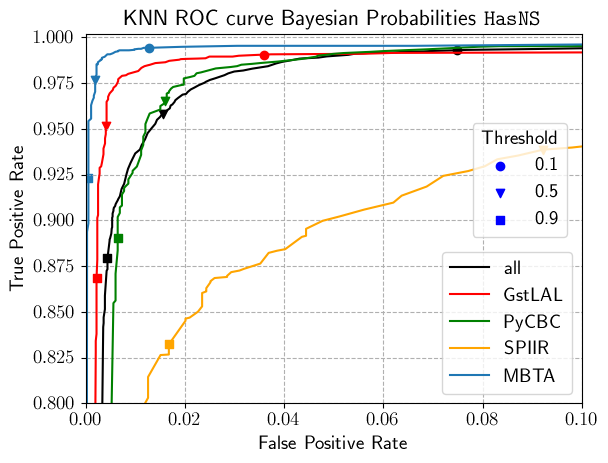
\includegraphics[width=0.45\linewidth]{roc_mdc_KNN_NS}
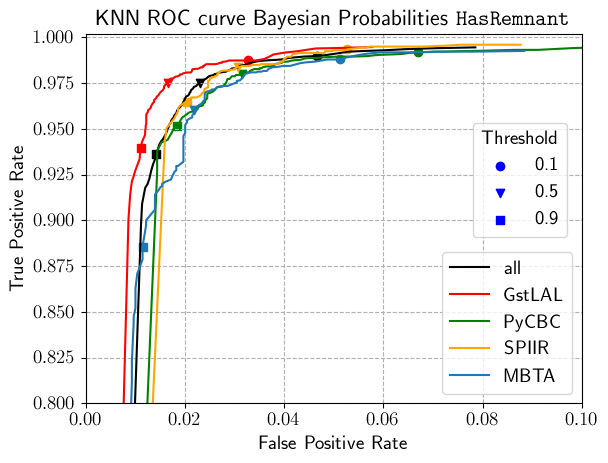
\includegraphics[width=0.45\linewidth]{roc_mdc_KNN_REM}
\caption{\ac{ROC} curves obtained from the \ac{O3} \ac{MDC} data set for the \ac{KNN} classifier (left: \hasns, right: \hasrem). The different \ac{LVK} matched-filtering pipelines are indicated by different colors (GstLAL: red; PyCBC: green; gold: SPIIR; blue: MBTA). The results for all pipelines are shown in black. The circle, triangle, and square markers denote probability thresholds of $0.1$, $0.5$, and $0.9$, respectively.}
\label{fig:rocMDC_KNN}
\end{figure*}

\begin{figure*}%[h]
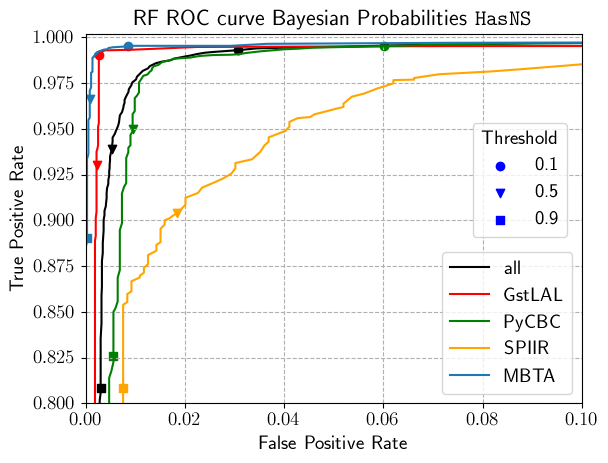
\includegraphics[width=0.45\linewidth]{roc_mdc_RF_NS}
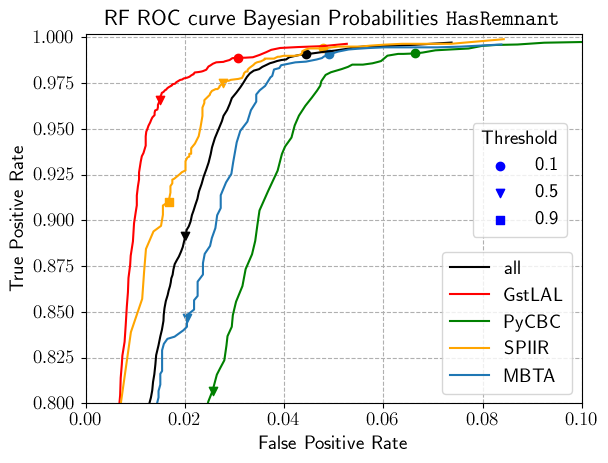
\includegraphics[width=0.45\linewidth]{roc_mdc_RF_REM}
\caption{\ac{ROC} curves obtained from the \ac{O3} \ac{MDC} data set for the \ac{RF} classifier (left: \hasns, right: \hasrem). The different \ac{LVK} matched-filtering pipelines are indicated by different colors (GstLAL: red; PyCBC: green; gold: SPIIR; blue: MBTA). The results for all pipelines are shown in black. The circle, triangle, and square markers denote probability thresholds of $0.1$, $0.5$, and $0.9$, respectively.}
\label{fig:rocMDC_RF}
\end{figure*}

Finally, we apply the method to derive Bayesian probabilities for the events in the \ac{LVK} \ac{GWTC3} catalog~\cite{LIGOScientific:2021djp}.  In Table~\ref{tab:real_data_bayesian} we
report the results for some of the most significant \ac{GWTC3} events, labeled with their event ID. The $P_M(\hasns |\bf{A_E})$ and $P_M(\hasrem |\bf{A_E})$ probabilities for GW170817 and
GW190425, the two confirmed \ac{BNS} detections are $\sim 1$ as expected.  The probabilities for GW190426 and GW200115 (\ac{NSBH} mergers) are $P_M(\hasns |{\bf{A_E}}) \sim 1$ and
$P_M(\hasrem |{\bf{A_E}}) < 10^{-3}$. The two remaining significant events with non-zero probabilities are GW190814 and GW190924. These events were reported as high mass-ratio BBH
mergers. 

The fact that the system's component masses differ greatly from one another can be used to explain why $P_M(\hasns |\bf{A_E})$ for these events is not zero. In particular, the discrepancy
between \ac{RF} and \ac{KNN} for GW190814 can be understood from the different ways the two algorithms operate. \ac{RF} applies hard cuts on decision trees to evaluate its outcome.
\ac{KNN} looks at the fractions of neighbors surrounding the event. The detection pipeline returned a secondary mass compatible with an \ac{NS} for three of the 23 \ac{EOS}. However,
since the region of the parameter space close to the mass gap, i.e., the region between high \ac{NS} masses and low \ac{BH} masses, is not well covered in the \ac{O2} training data set,
\ac{KNN} overestimates the effect of the three \ac{EOS} predicting a secondary mass in the \ac{NS} region. 

\begin{table}[]
\begin{tabular}{c|cc|cc}
\hline
\multicolumn{1}{c|}{}      & \multicolumn{2}{c|}{$P_M(\hasns|{\bf A}_{\bf E})$}                                                & \multicolumn{2}{c}{$P_M(\hasrem|{\bf A}_{\bf E})$}                                                \\ \hline
\multicolumn{1}{c|}{event ID}   & \multicolumn{1}{c}{RF} & \multicolumn{1}{c}{KNN}  & \multicolumn{1}{c}{RF} & \multicolumn{1}{c}{KNN} \\ \hline
GW170817                                   & 0.998                   & 0.989                    & 0.997                   & 0.985                                  \\
GW190425                                   & 0.998                   & 0.989                    & 0.997                   & 0.985                            \\
GW190426                                   & 0.997                   & 0.985                    & $< 10^{-3}$             & $< 10^{-3}$                    \\
GW190814                                   & 0.042                   & 0.567                   & $< 10^{-3}$              & $< 10^{-3}$                      \\
GW190924                                   & 0.012                   & 0.054                   & $< 10^{-3}$              & $< 10^{-3}$                       \\               
GW200115                                   & 0.998                   & 0.989                   & $< 10^{-3}$              & $< 10^{-3}$                           \\
\hline
\end{tabular}
\caption{Bayesian probabilities of a few significant \ac{GW} events from the \ac{GWTC3} catalog. GW170817 and GW190425, GW190426 and GW200115, and GW190814 and GW190924 were determined to be \ac{BNS}, \ac{NSBH}, and \ac{BBH} mergers, respectively. The probability values in the table are rounded to three decimal figures.}
\label{tab:real_data_bayesian}
\end{table}

Figures~\ref{fig:param_sweep_KNN} and~\ref{fig:param_sweep_RF} show parameter sweeps in the space of the binary component masses for the \ac{KNN} and \ac{RF} Bayesian probabilities,
respectively. Different rows correspond to different values of the component spins. Both algorithms perform in a similar way for $P_M(\hasns |\bf{A_E})$. However, the parameter sweeps for
$P_M(\hasns |\bf{A_E})$ for \ac{KNN} are noisier than \ac{RF} for large primary masses. As was noted above, the \ac{KNN} algorithm operates by looking at the closest neighbors. If
neighbors with different labels are present in the region of interest, the outcome is bound to be noisy. The \ac{RF} algorithm applies hard selection cuts to primary masses. This results
in a more uniform probability. Changes in spin seem to not significantly affect the outcome.  Similar behaviors for \ac{KNN} and \ac{RF} can also be observed in the case of $P_M(\hasrem
|\bf{A_E})$. As expected from the Foucart formula, $P_M(\hasrem |\bf{A_E})$ increases with the primary mass for large primary spins, and the region with $P_M(\hasrem |\bf{A_E}) \sim 1$ is
included in the region where $P_M(\hasns |\bf{A_E}) \sim 1$.

\begin{figure*}%[h]
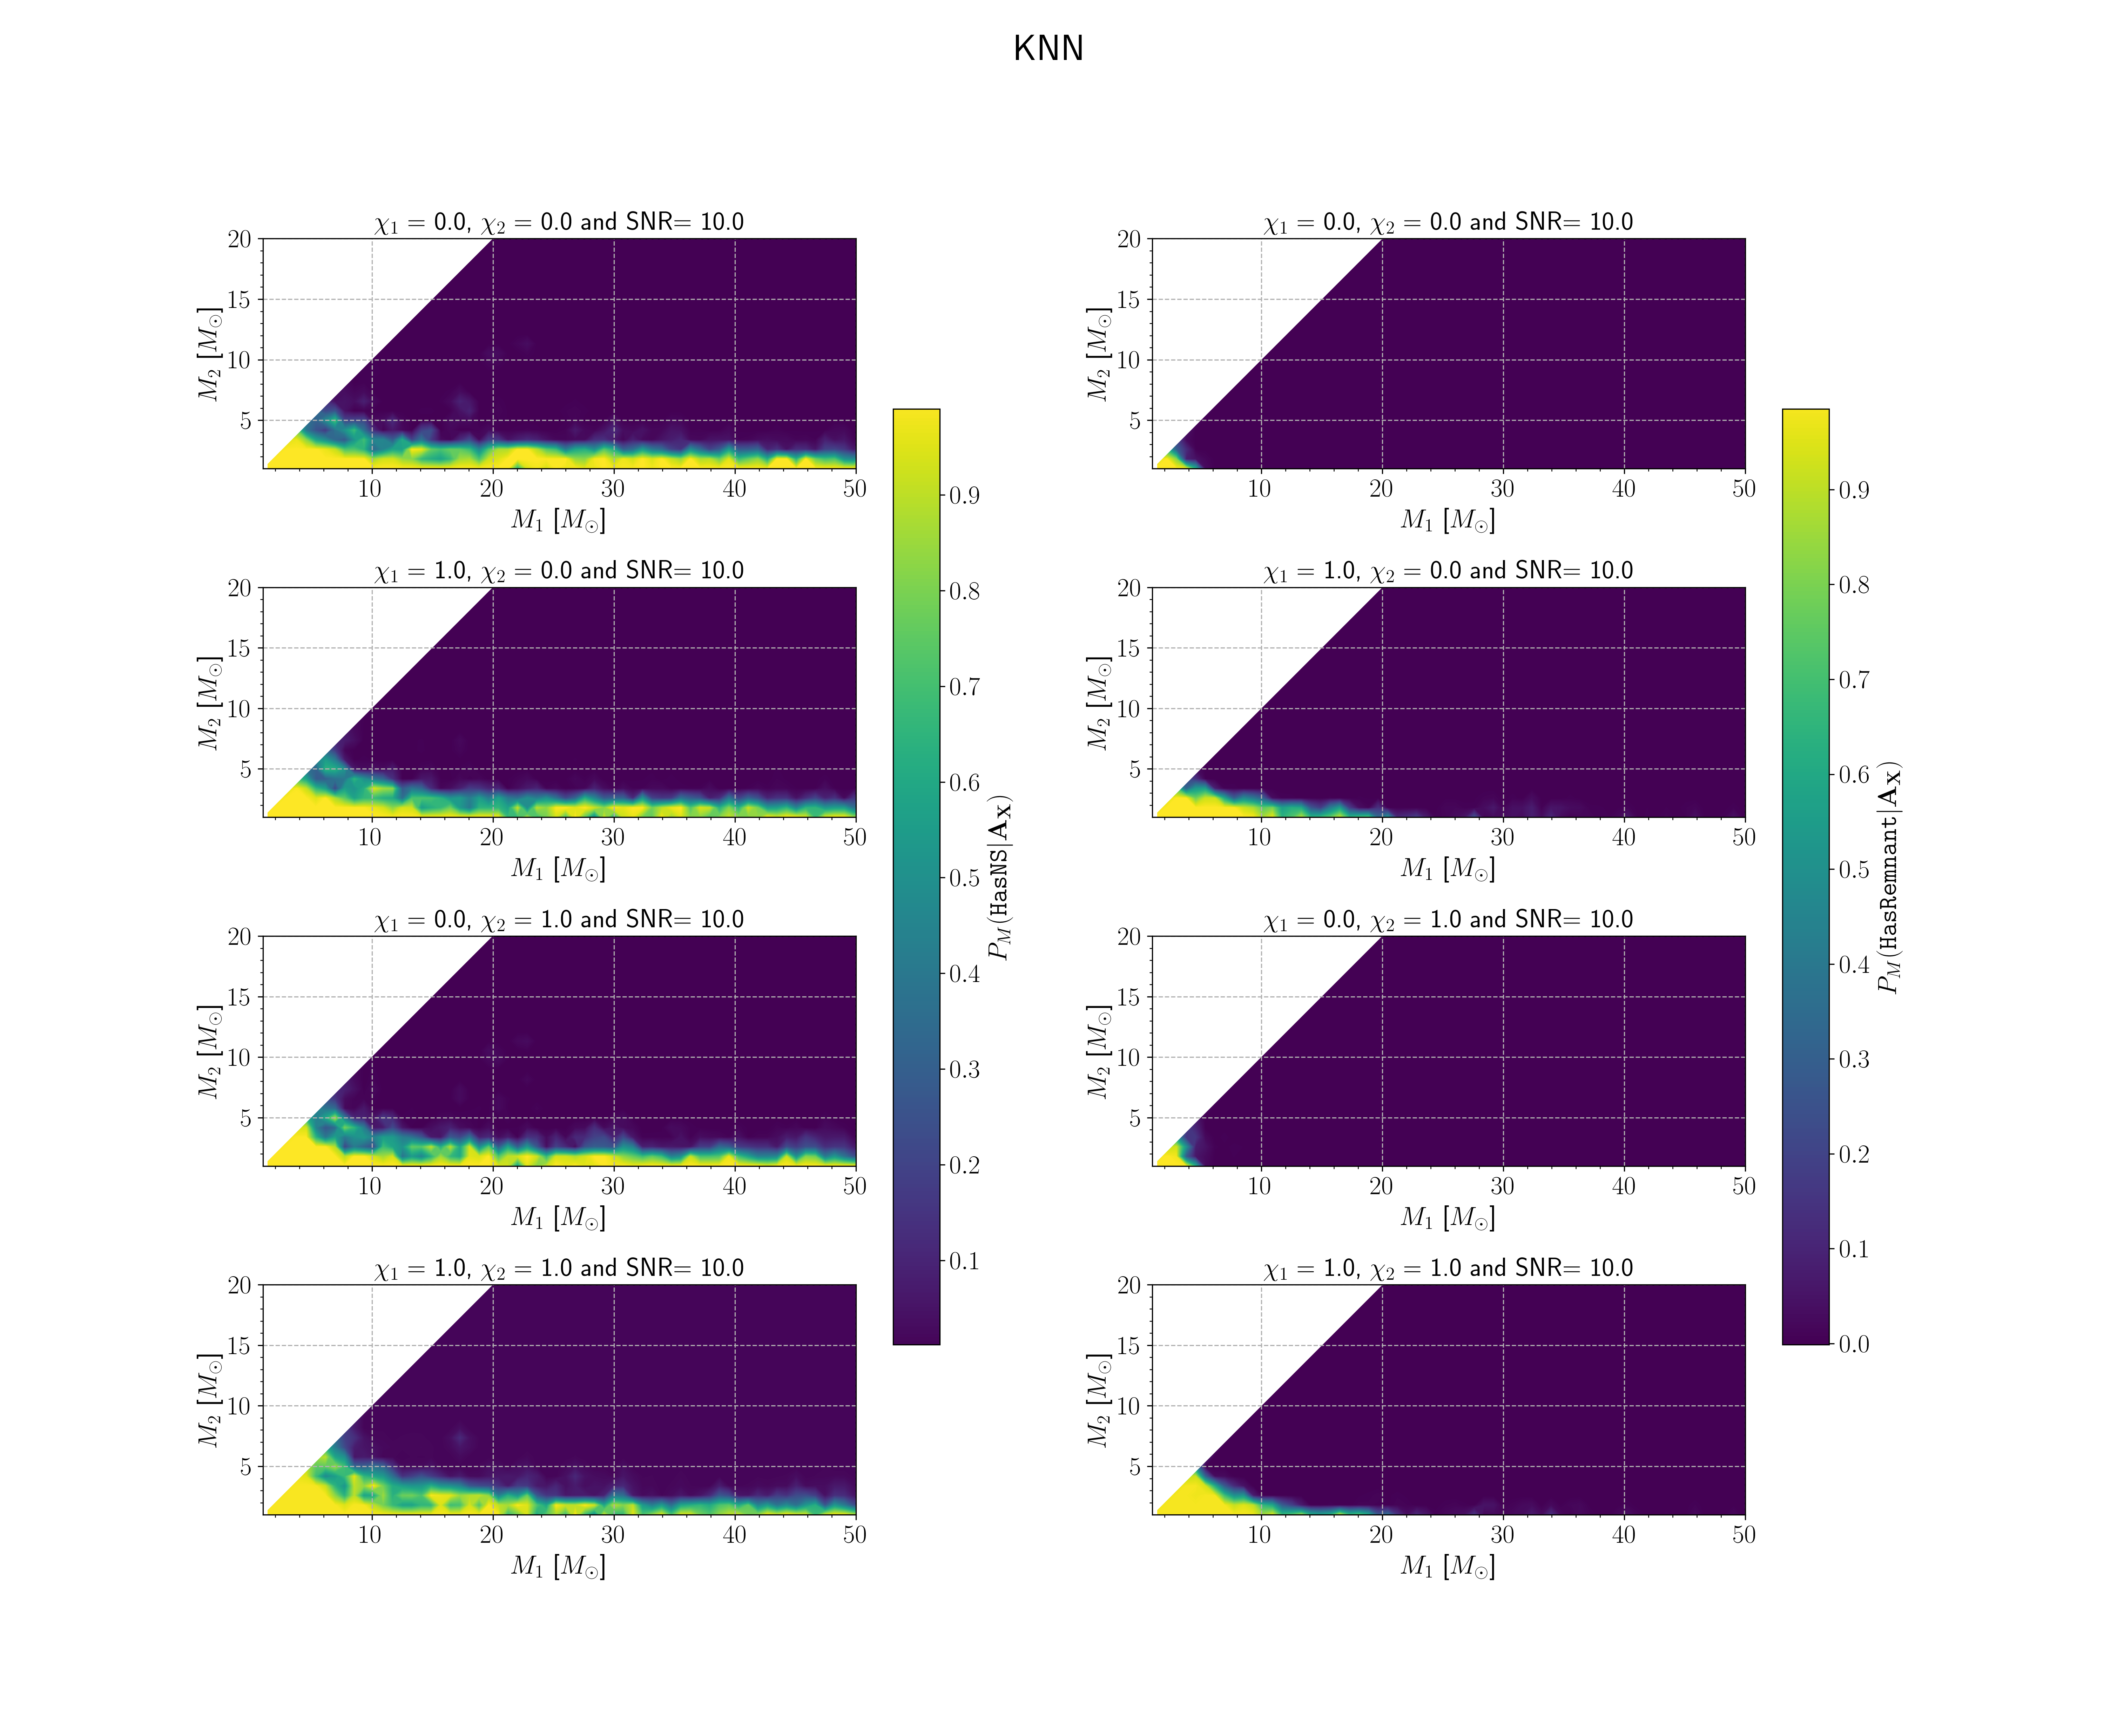
\includegraphics[width=0.9\linewidth]{KNN_parameter_sweep}
    \caption{Parameter sweeps for $P_M(\hasns |\bf{A_E})$ (left panels) and $P_M(\hasrem |\bf{A_E})$ (right panels) for the \ac{KNN} algorithm. $M_1$ and $M_2$ are the primary and secondary component masses of the binary. $\chi_1$ and $\chi_2$ are their effective spins. The \ac{SNR} is fixed to 10.}
\label{fig:param_sweep_KNN}
\end{figure*}

\begin{figure*}%[h]
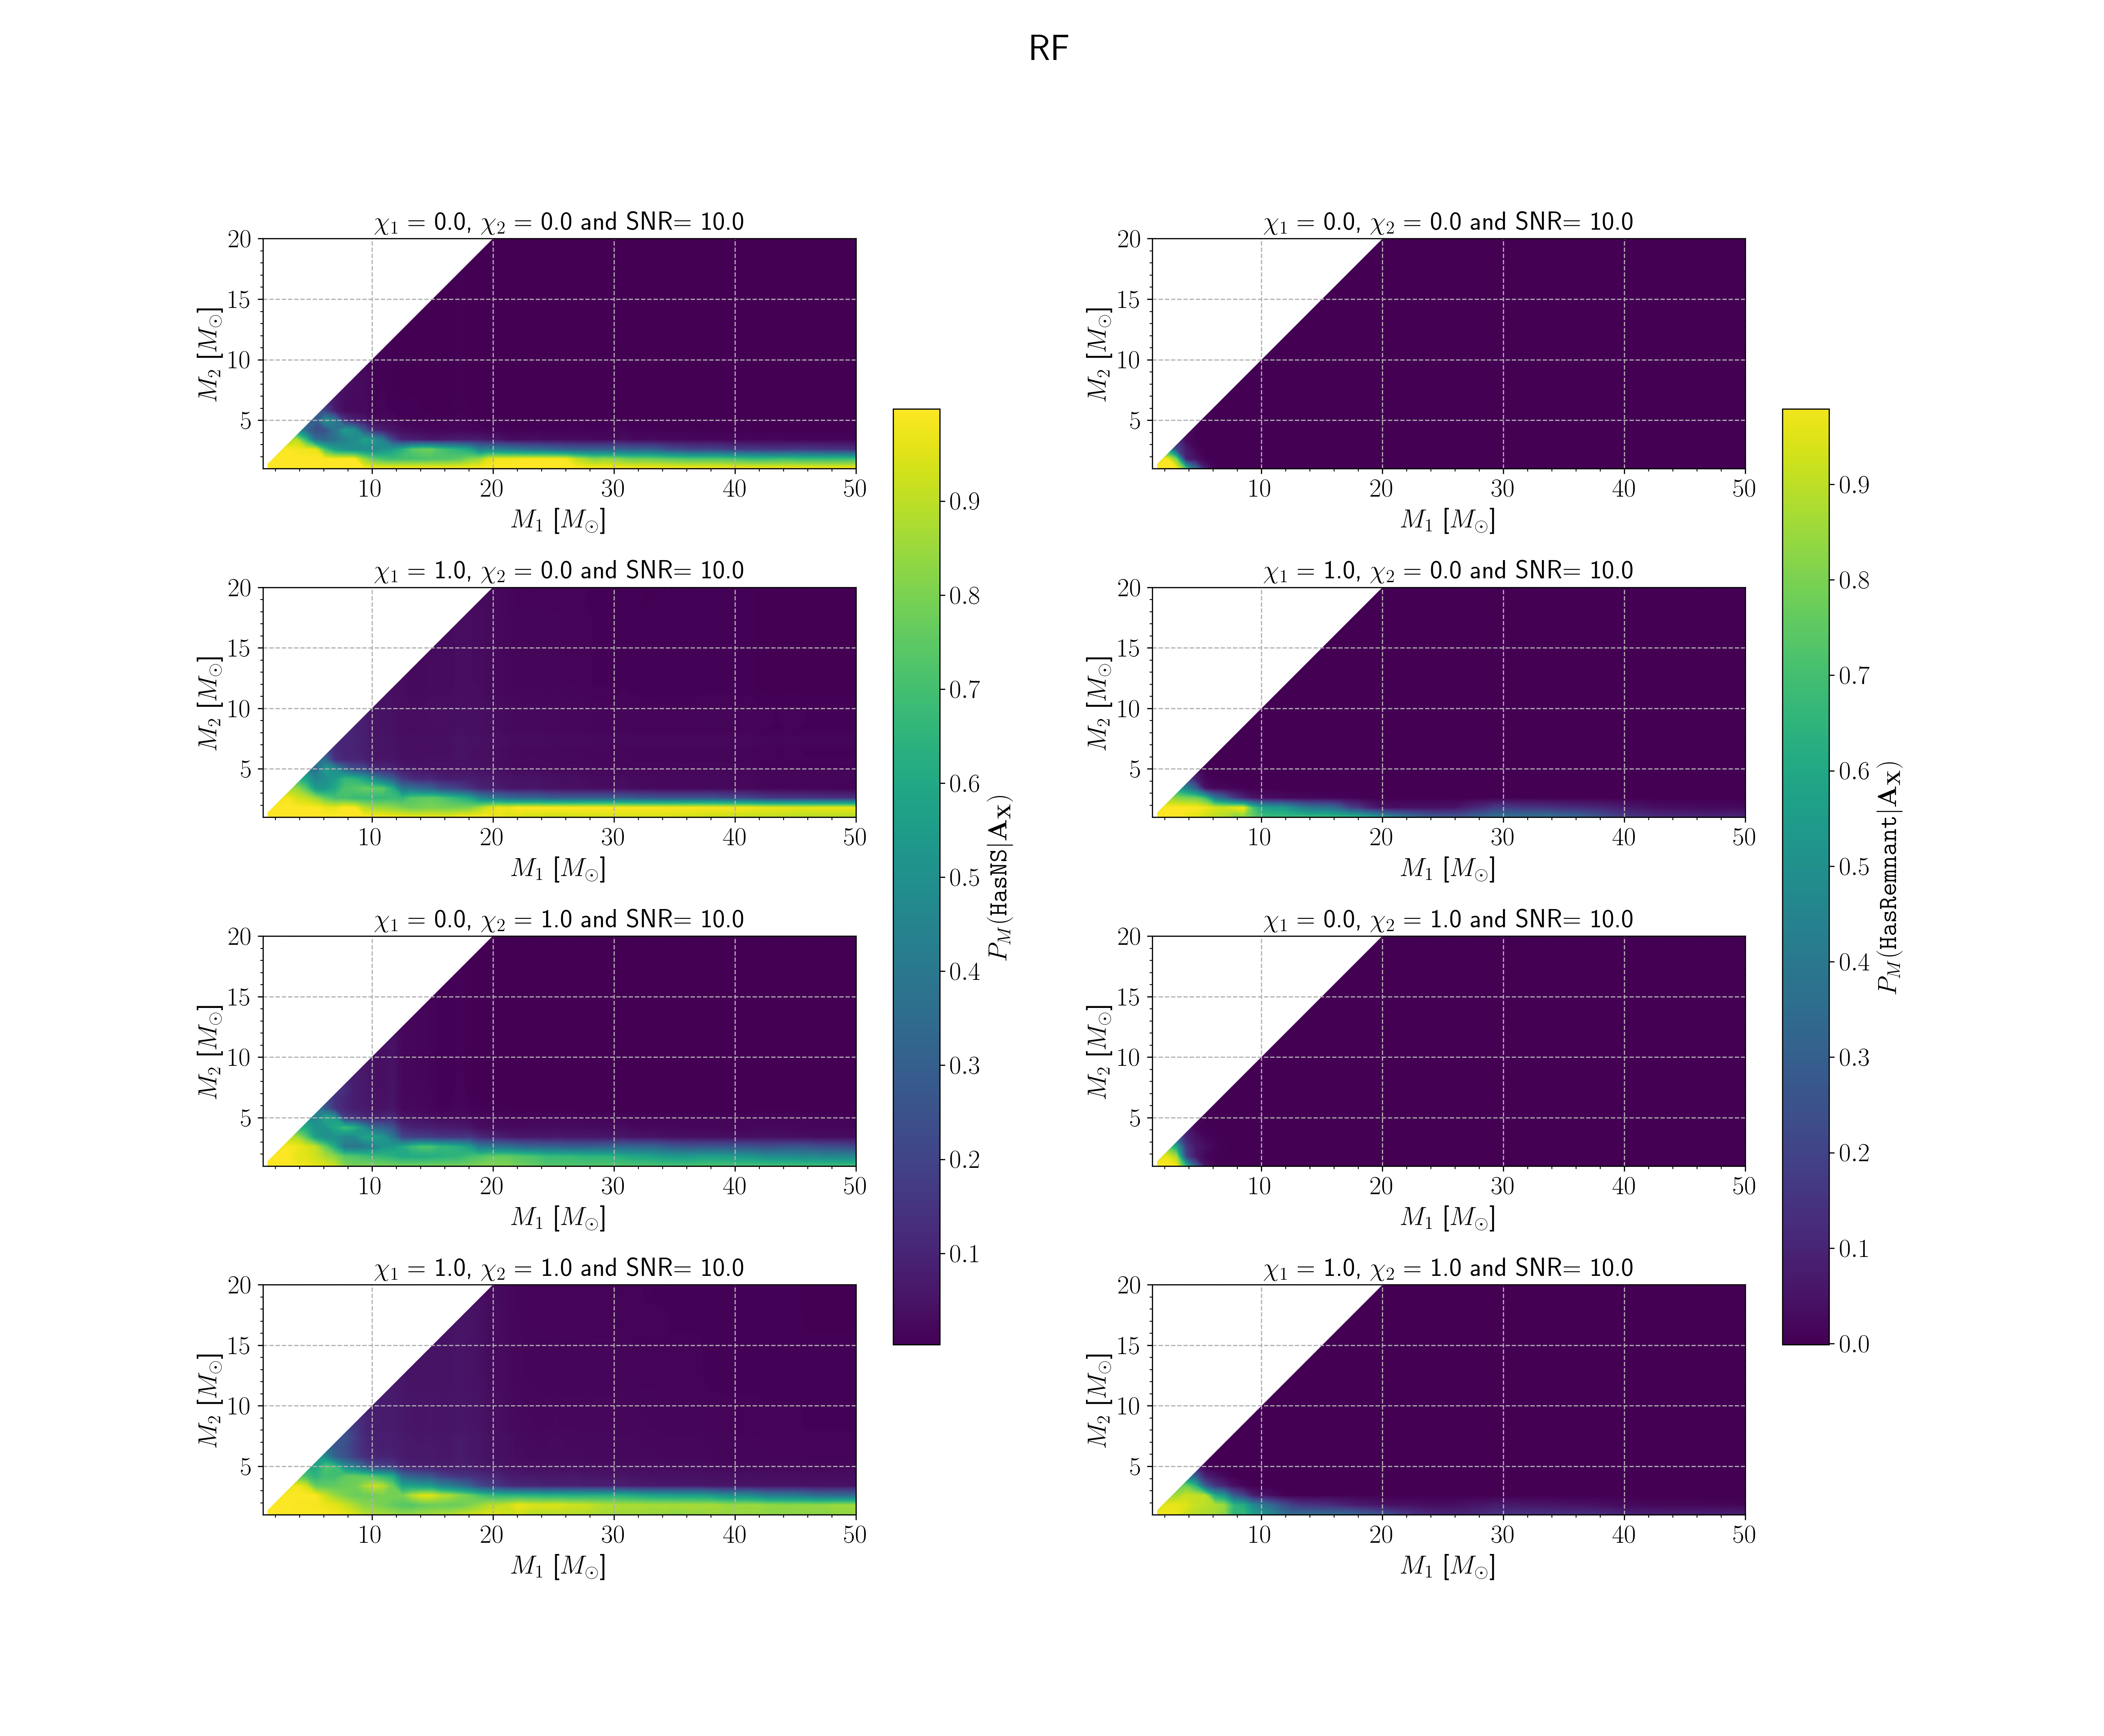
\includegraphics[width=0.9\linewidth]{RF_parameter_sweep}
    \caption{Parameter sweeps for $P_M(\hasns |\bf{A_E})$ (left panels) and $P_M(\hasrem |\bf{A_E})$ (right panels) for the \ac{RF} algorithm. $M_1$ and $M_2$ are the primary and secondary component masses of the binary. $\chi_1$ and $\chi_2$ are their effective spins. The \ac{SNR} is fixed to 10.}
\label{fig:param_sweep_RF}
\end{figure*}
